\documentclass[12pt]{article}
\usepackage[utf8]{inputenc}
\usepackage[margin=0.5in]{geometry}
\usepackage{bm}
\usepackage{graphicx}
\usepackage[rightcaption]{sidecap}
\usepackage{hyperref}

\title{MEG Analysis Documentation}

\author{Henry Allen}

\begin{document}

\maketitle

\section{MEG Analysis}
\subsection{Preprocessing}

MEG analysis was performed in Python with the MNE package. Analysis was performed
on 204 planar gradiometers (the 102 magnetometers were not used for analysis). Epochs were rejected
for a subject if maximum peaks for any gradiometer exceeded a threshold of $4000\times10^{-13}  \frac{T}{m}$.
MEG data was then band-pass filtered from 2-40hz, removing any potential low-frequency artifacts and
unused high-frequency data.

The Independent Component Analysis (ICA) for each subject was calculated to remove artifacts caused
by EMG and EOG artifacts. ICA performs source separation for statistically independent components of signals.
Eighty Independent components were generated for each subject, and independent components resembling
EMG and EOG artifacts were visually selected and then excluded from the filtered MEG dataset.

Trials were epoched at the onset of the the gabor patch stimulus. Trials were performed in
batches of 100 trials that were concatenated together for each subject.

\begin{figure}[h]
  \centering
  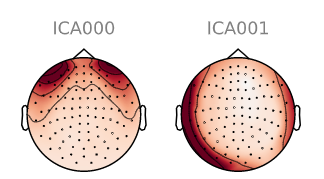
\includegraphics{ica_figure.PNG}
  \caption{Example ICA components chosen for exclusion. The left component represents
  artifacts resulting from eye blinks, while the right component represents muscle
  movements from the head that we wish to exclude}
\end{figure}


\subsection{ERF Analysis}
The averaged evoked responses for each subject were measured to ensure that visual responses
appeared in the occipital area as expected. Time-locked epoch responses were averaged over all
trial blocks for each subject at each electrode and visually analyzed for aberrations.

\begin{figure}[h]
  \centering
  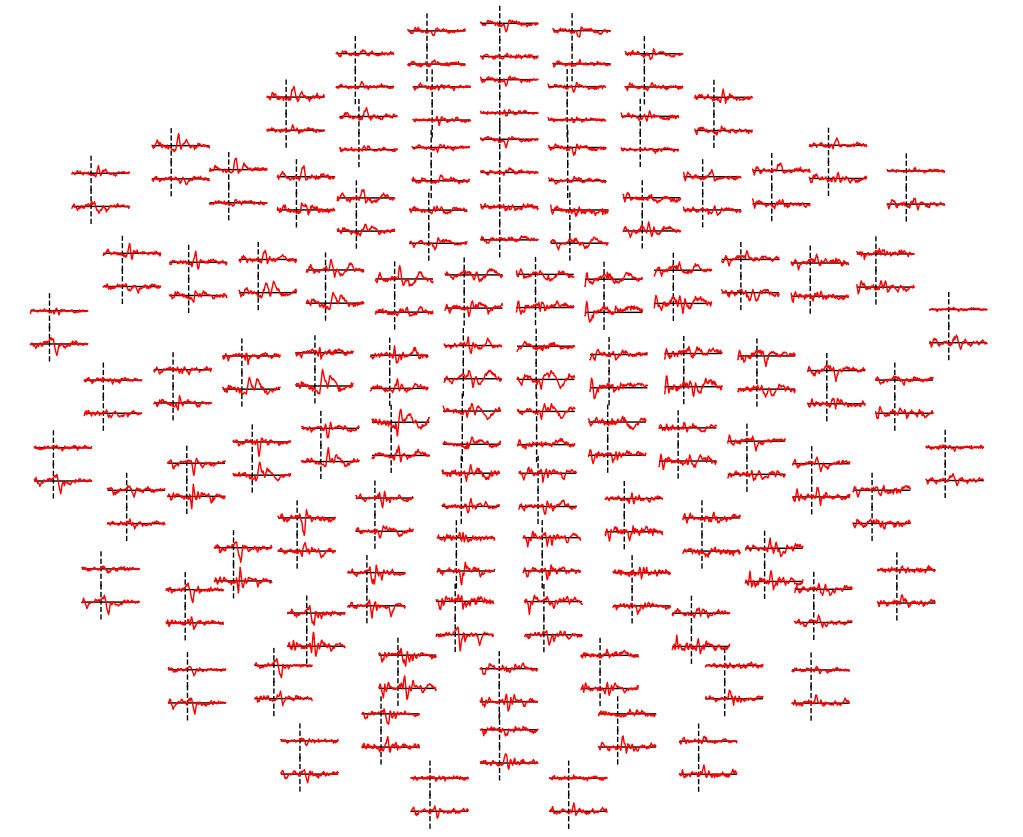
\includegraphics[scale=0.8]{good_topomap.PNG}
  \caption{In a good subject, like the one above, we get evoked responses in left hemisphere
  occipital and temporal electrodes around 0.2 seconds after the stimulus is shown. The stimulus
  was only shown in the right visual field, so we see limited activation in the right
  hemisphere.}
  
\end{figure}

\end{document}